\documentclass{beamer}
\usepackage{amssymb,amsmath,mathrsfs}

\newcommand{\showtoc}{
  \frame{
    \frametitle{Overview}
    \tableofcontents[sectionstyle=show/shaded,subsectionstyle=hide]
  }
}

\usepackage[PostScript]{diagrams}

\usepackage{epsfig,psfrag,epstopdf}

\newcommand{\sQ}{\mathcal{Q}}
\newcommand{\nc}{\mathit{nc}}
\DeclareMathOperator*{\argmin}{arg\,min}

%\usetheme{PaloAlto}
\usetheme{Szeged}
%\usecolortheme{beaver}

\usepackage{graphicx}
\graphicspath{{./figures/}}
\DeclareGraphicsExtensions{.pdf,.eps}

\usepackage{prelim_def}

\usepackage{media9}
\addmediapath{videos}

\newtheorem{massump}{Modeling Assumptions}

\title[Energy Shaping]{A Lyapunov Approach to Orbital \\Stabilization through Energy Shaping}
\subtitle{Applications to Bipedal Walking\\--- Preliminary Results ---}
\author{R. W. Sinnet}
\institute{Department of Mechanical Engineering\\ Texas A\&M University}
\date{Monday, June 30, 2014}


\begin{document}

\frame{\titlepage}

\begin{frame}
  \frametitle{Overview}
  \tableofcontents[sectionstyle=show,subsectionstyle=hide]
\end{frame}

\section{Introduction}
\showtoc

\subsection{Motivation}
\begin{frame}
  \frametitle{Goal}
  goal
\end{frame}

%\subsection{History}
\begin{frame}[t]
  \only<1> {
    {\Large \bf Biomechanics}
    \begin{itemize}
    \item
      D.~A. Winter, {\em Biomechanics and Motor Control of Human Movement}, 2nd ed., New York: Wiley-Interscience, 1990.\\
    \item
      J. Perry and J. Burnfield, Gait Analysis: Normal and Pathological Function, 2nd ed., Thorofare: Slack Inc., 2010.\\
    \end{itemize}
  }
  \only<2,3> {
    \textcolor{gray}{\Large \bf Biomechanics}\\[1mm]
  }

  \only<2> {
    {\Large \bf Reduction-Based Control}
    \begin{itemize}
    \item
      A.~D. Ames et al., {\em On the Geometric Reduction of Controlled Three-Dimensional Bipedal Robotic Walkers}, in 3rd Workshop on Lagrangian and Hamiltonian Methods for Nonlinear Control (LHMNL'06), Nagoya, Japan, Jul. 2006.\\
    \item
      R.~W. Sinnet et al., {\em 3D Bipedal Walking with Knees and Feet: A Hybrid Geometric Approach}, in 48th IEEE Conference on Decision and Control, Shanghai, P. R. China, Dec. 2009.
    \item
      R~.W. Sinnet and A.~D. Ames, {\em Bio-Inspired Feedback Control of Three-Dimensional Humanlike Bipedal Robots}, in Journal of Robotics and Mechatronics, special issue on {\em Focused Areas and Future Trends in Bio-Inspired Robots}, Aug. 2012.

    \end{itemize}
  }
  \only<1,3> {
    \textcolor{gray}{\Large \bf Reduction-Based Control}\\[1mm]
  }

  \only<3> {
    {\Large \bf Human-Inspired Control}
    \begin{itemize}
    \item
      A.~D. Ames, {\em First Steps Toward Automatically Generating Bipedal Robotic Walking from Human Data}, in 8th International Workshop on Robotic Motion and Control, Gron{\'o}w, Poland, Jun. 2011.
    \item
      R.~W. Sinnet et al., {\em A Human-Inspired Hybrid Control Approach to Bipedal Robotic Walking}, in 18th IFAC World Congress (IFAC 2011), Milan, Italy, Sep. 2011.
    \item
      R.~W. Sinnet et al., {\em A Human-Inspired Framework for Bipedal Robotic Walking Design}, International Journal of Biomechatronics and Biomedical Robotics, Jan. 2014.
    \end{itemize}
  }
  \only<1,2> {
    \textcolor{gray}{\Large \bf Human-Inspired Control}
  }

\end{frame}

\begin{frame}
  \frametitle{History}
  \begin{columns}

    \begin{column}{.24\textwidth}
      \textcolor{blue}{Passive Walking:}
      \begin{figure}
        \centering
        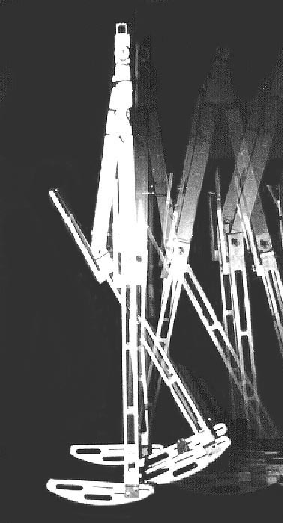
\includegraphics[height=4.5cm]{bipeds_ruina}
      \end{figure}
    \end{column}

    \begin{column}{.24\textwidth}
      \textcolor{blue}{Passivity-Based Control:}
      \begin{figure}
        \centering
        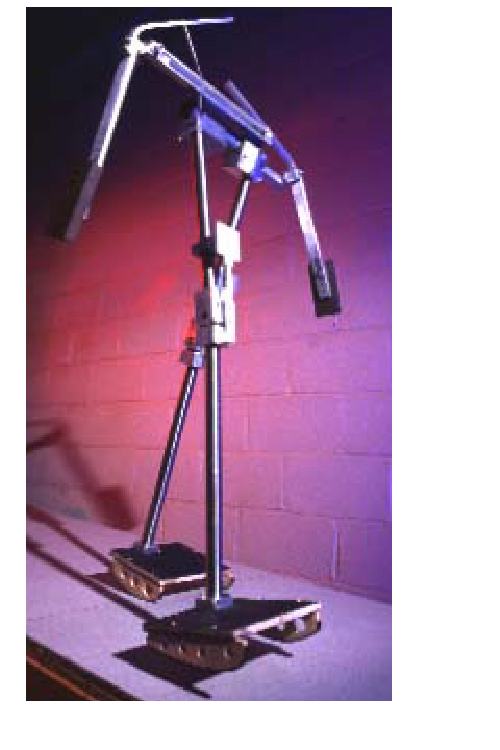
\includegraphics[height=4.5cm]{bipeds_collins}
      \end{figure}
    \end{column}

    \begin{column}{.24\textwidth}
      \textcolor{blue}{Hybrid Zero Dynamics:}
      \begin{figure}
        \centering
        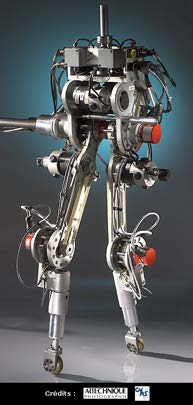
\includegraphics[height=4.5cm]{figures/bipeds_grizzle}
      \end{figure}
    \end{column}

    \begin{column}{.24\textwidth}
      \textcolor{blue}{Human-Inspired Control:}
      \begin{figure}
        \centering
        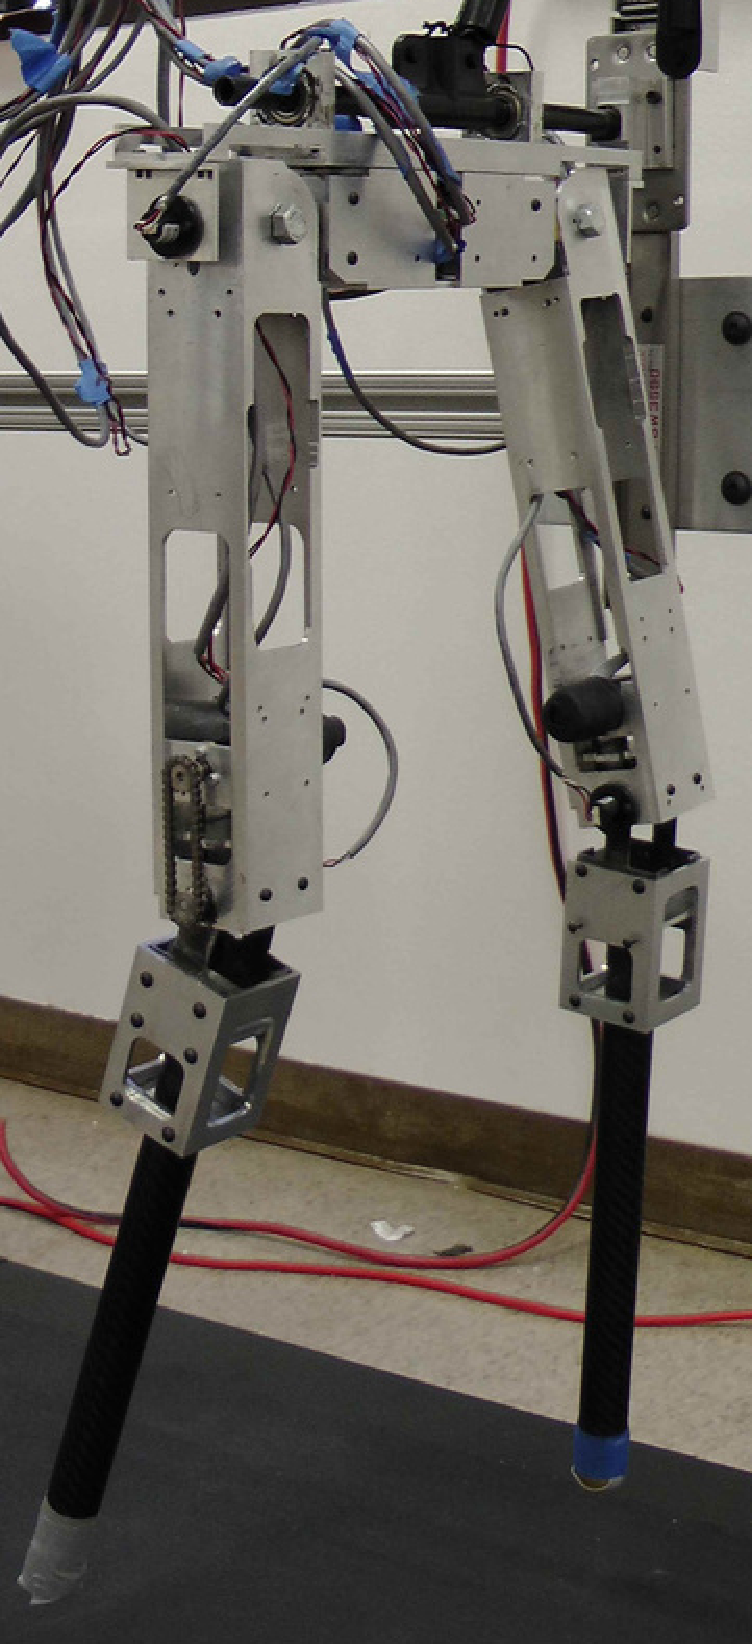
\includegraphics[height=4.5cm]{figures/bipeds_ames}
      \end{figure}
    \end{column}

  \end{columns}
\end{frame}

%%%%%%%%%%%%%%%%%%%%%%%%%%%%%%%%%%%%%%%%%%%%%%%%
%%%%%%%%%%%%%%%%%%%%%%%%%%%%%%%%%%%%%%%%%%%%%%%%
%%%%%%%%%%%%%%%%%%%%%%%%%%%%%%%%%%%%%%%%%%%%%%%%

\section{Mechanics}
\showtoc

\subsection{Hybrid Systems}
\begin{frame}
  \frametitle{Bipedal Models}
  \begin{figure}
    \centering
    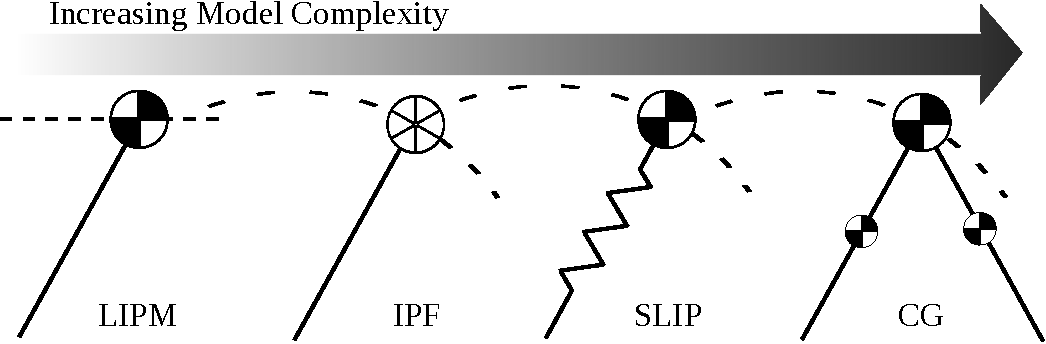
\includegraphics[width=.9\textwidth]{biped-models}
  \end{figure}
  \begin{itemize}
  \item Bipedal locomotion has been studied with a variety of models.
  \item Pendulum models consider massless legs with no impacts.
  \item Kinematic chains are markedly more complex than pendula.
  \end{itemize}
\end{frame}

\begin{frame}
  \frametitle{Modeling Hybrid Systems}
  \begin{columns}
    \begin{column}{.63\textwidth}
      \begin{definition}
        A \alert{hybrid control system} is a tuple \vspace{-.3cm}
        $$\HCS = \hcsystem, \vspace{-.4cm}$$
        where
        \begin{itemize}
        \item
          $\Domain \subset \mathcal{X}$ is the {\em domain of admissiblity} with state space $\mathcal{X}$,
        \item
          $\ControlSet$ is a set of {\em admissible controls},
        \item
          $\Guard$ is a {\em guard} or {\em switching surface},
        \item
          $\ResetMap$ is a smooth {\em reset map},
        \item
          $(f, g)$ is a control system on $\Domain$: \vspace{-3mm}
          \begin{align*}
            \dot{x} = f(x) + g(x) \, u.
          \end{align*}
        \end{itemize}
      \end{definition}
    \end{column}
    \begin{column}{.4\textwidth}
      \begin{figure}
        \centering
        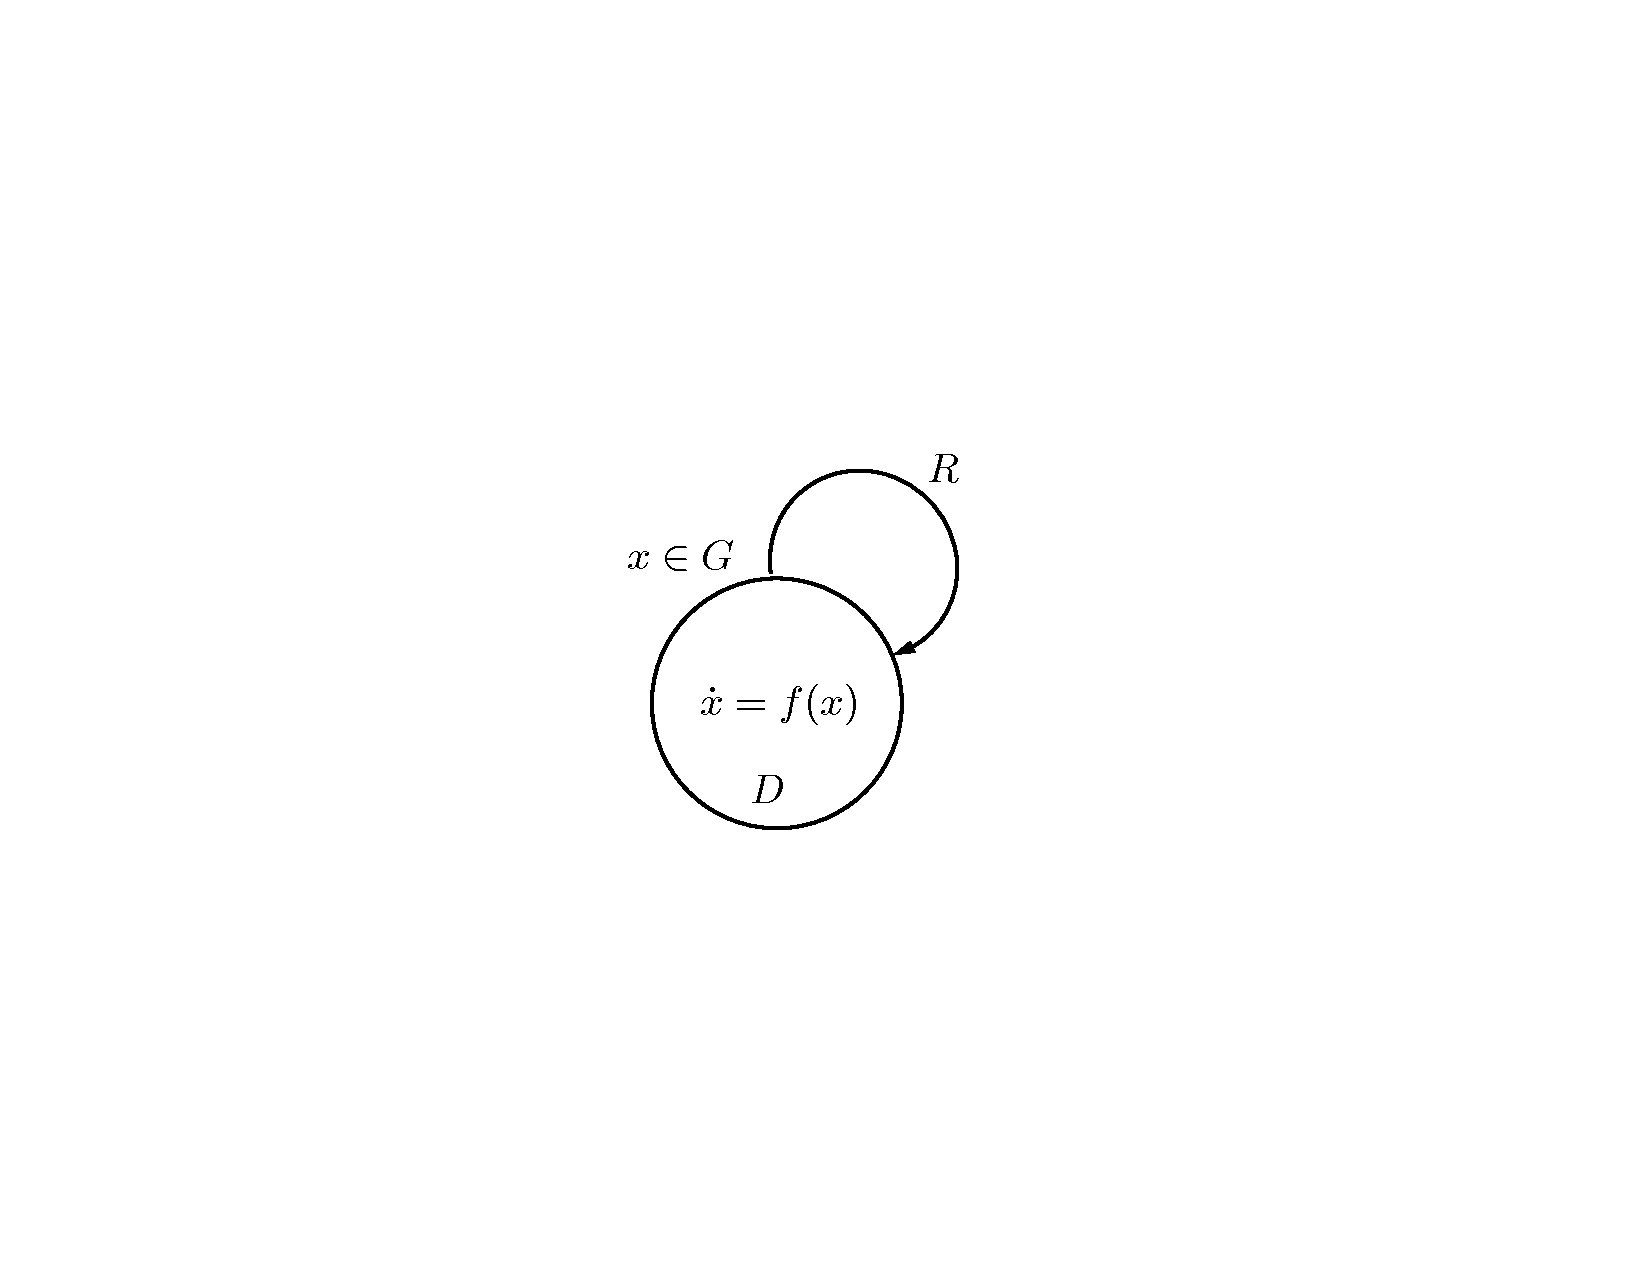
\includegraphics[width=.9\textwidth]{hsystem}\\
      \end{figure}
      A \textcolor{blue}{simple hybrid system}:\vspace{-.3cm}
      $$\HS = \hsystem$$
    \end{column}
  \end{columns}
\end{frame}

\begin{frame}
  \frametitle{Lagrangian Systems}
  Mechanical systems are defined by:
  \begin{itemize}
  \item Kinetic energy, $T : T\sQ \to \R^+$,\\
  \item  Potential energy, $U : \sQ \to \R$,
  \end{itemize}
  which together comprise the total energy,
  \begin{align*}
    E(q, \dot q) = T(q, \dot q) + U(q).
  \end{align*}
  In a Hamiltonian system, energy is conserved and thus the dynamics reflects the flow of energy between $T(q, \dot q)$ and $U(q)$.
\end{frame}

\begin{frame}
  \frametitle{Swing Phase Dynamics}
  \begin{columns}
    \begin{column}{.55\textwidth}
      For Lagrangian $\Lagrangian$ with coordinates
      \begin{align*}
        x = (\q^{T}, \dq^{T})^{T} \in T\ConfigurationSpace,
      \end{align*}
      the principal of least action allows one to construct a dynamic model:
      \begin{align*}
        \D(\q) \, \ddq + \C(\q, \dq) \, \dq + \G(\q) = B(\q) \, u,
      \end{align*}
      or $\dot x = f(q, \dot q) + g(q) \, u,$ with
      \begin{align*}
        f(\q, \dq) &= \left(\!\!\begin{array}{c}
        \dq\\
        \D^{-1}(\q) (-\C(\q, \dq) \, \dq - \G(\q))
        \end{array}\!\!\right),\\
        g(\q) &= \left(\!\!\begin{array}{c}
        \mathbf{0}_{m \times m}\\
        \D^{-1}(\q) B(\q)
        \end{array}\!\!\right).
      \end{align*}
    \end{column}\!\!
    \begin{column}{.45\textwidth}
      \begin{figure}
        \centering
        \vspace{-10mm}
        \caption{Physical configuration}
        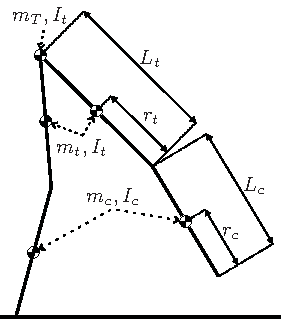
\includegraphics[width = 1.0\columnwidth]{robot_config}
      \end{figure}
    \end{column}
  \end{columns}
\end{frame}

\begin{frame}
  \frametitle{Impact Dynamics}
  Introduce extended coordinates $\qe = (p_{x}, p_{y}, p_{z}, \q^{T})^{T} \in \R^{3} \times \ConfigurationSpace$. Angular momentum balance based on H{\"u}rm{\"u}zl{\"u} and Marghitu:
  \begin{massump}
    \begin{itemize}
    \item Rigid-body plastic impacts
    \item Enough friction to prevent slipping
    \item Impact points do not rebound
    \item Motors do not produce impulses
    \item No instantaneous change in configuration, i.e., $\qe^{-} = \qe^{+}$
    \end{itemize}
  \end{massump}
  Under these assumptions, the discrete dynamics satisfies
  \begin{align*}
    \left[\begin{array}{c c}
        \D_{e}(\qe) & -\Jacobian^{T}(\qe)\\
        \Jacobian(\qe) & \mathbf{0}_{3 \times 3}
      \end{array}\right]
    \left[\begin{array}{c}
        \dq^{+}\\
        \delta F(\qe, \dqe)
      \end{array}\right]
    = \left[\begin{array}{c c}
        \D_{e}(\qe) \, \dqe^{-}\\
        \mathbf{0}_{3}
      \end{array}\right].
  \end{align*}
\end{frame}

\subsection{Solutions to Hybrid Systems}
\begin{frame}
  \frametitle{Solutions to Dynamical Systems}
  dsys
\end{frame}

\begin{frame}
  \frametitle{Periodic Orbits}
\end{frame}

\begin{frame}
  \frametitle{Conservative Systems}
  csys
\end{frame}


\begin{frame}
  \frametitle{The Simplest Example: Passive Compass-Gait Biped}
  \only<1>{
    \begin{columns}
      \column{1.5in}
      Dynamic Model:
      \begin{align*}
        M(q) \ddot q + H(q, \dot q) = 0
      \end{align*}
      Control Law:
      \begin{align*}
        u = 0.
      \end{align*}
      \column{1.5in}
      \begin{figure}%width=1.0\columnwidth,
        
        \centering
        \def\svgwidth{1.0\columnwidth}
        \input{figures/cg2d-slope-model.eps_latex}
        \vspace{-2em}
        \caption{Compass-gait biped falling down a slope.}
      \end{figure}
    \end{columns}
  }

  \only<2>{
    \begin{figure}
      \includemedia[
        %width=1.0\columnwidth,
        %height=0.5625\columnwidth,
        width=1.0\columnwidth,
        height=0.5\columnwidth,
        addresource=cg2d_2link_simulation.mp4,
        activate=pageopen,
        flashvars={source=cg2d_2link_simulation.mp4&loop=true&autoPlay=true}
      ]{}{VPlayer9.swf}
      \caption{Stable passive gaits can be found for a range of slopes.}
    \end{figure}    
  }

  \only<3>{
    \begin{figure}
      \centering
      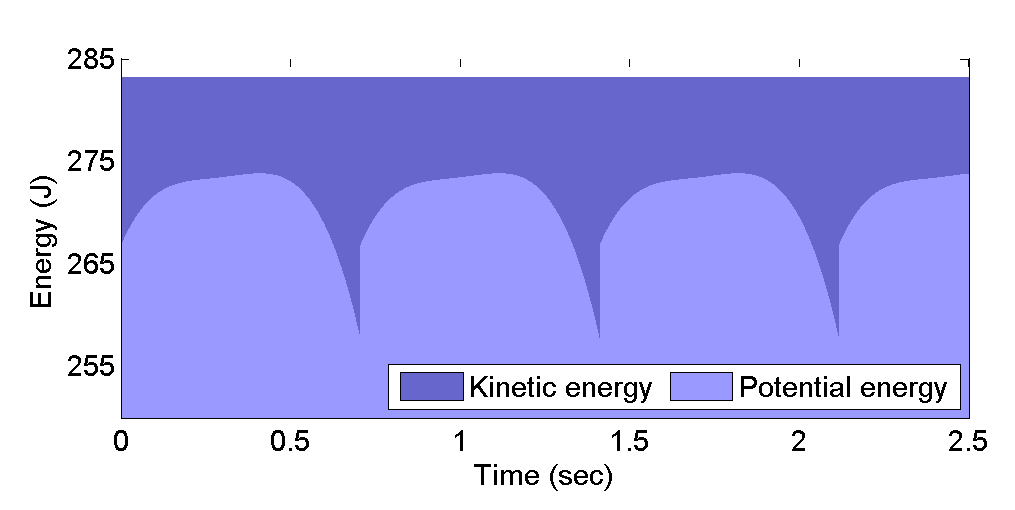
\includegraphics[width=1.0\columnwidth]{energy_cg2d_slope_model}
      \caption{Energy is exchanged between kinetic and potential in form.}
    \end{figure}    
  }
\end{frame}

\begin{frame}
  \frametitle{Example: Active Compass-Gait Biped}
  \only<1>{
    \begin{columns}
      \column{1.5in}
      Dynamic Model:
      \begin{align*}
        M(q) \ddot q + H(q, \dot q) = 0
      \end{align*}
      Control Law:
      \begin{align*}
        u &= G(q) - G(\Psi(q)).
      \end{align*}

      \column{1.5in}
      \begin{figure}
        \centering
        \def\svgwidth{1.0\columnwidth}
        \input{figures/cg2d-2link-model.eps_latex}
        \vspace{-2em}
        \caption{Compass-gait biped with Controlled Symmetries.}
      \end{figure}
    \end{columns}
  }
  \only<2>{
    \begin{figure}
      \includemedia[
        %width=1.0\columnwidth,
        %height=0.5625\columnwidth,
        width=1.0\columnwidth,
        height=0.5\columnwidth,
        addresource=cg2d_2link_simulation.mp4,
        activate=pageopen,
        flashvars={source=cg2d_2link_simulation.mp4&loop=true&autoPlay=true}
      ]{}{VPlayer9.swf}
      \caption{Passive downhill gaits can be translated to flat ground with Controlled Symmetries.}
    \end{figure}    
  }
  \only<3>{
    \begin{figure}
      \centering
      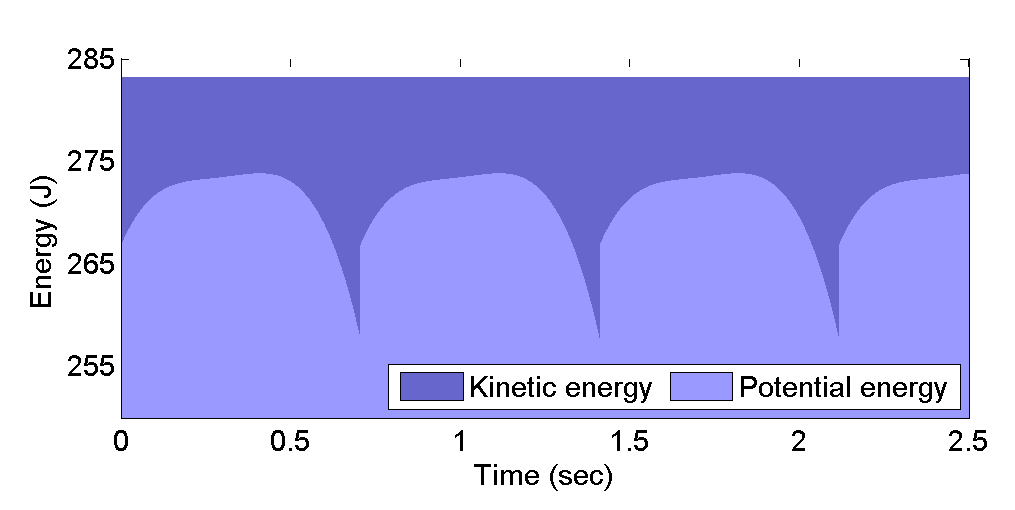
\includegraphics[width=1.0\columnwidth]{energy_cg2d_slope_model}
      \caption{Energy of the shaped system is conserved.}
    \end{figure}    
  }
\end{frame}

\begin{frame}
  \frametitle{Nonconservative Systems}
  For a nonconservative system, energy flows out of the system at a rate of $F_{\nc} \cdot dq$. Thus, the following quantity is conserved:
  \begin{align*}
    E_{c} &= T(q, \dot q) + U(q) - \int_{t_{0}}^{t_{1}} \! F_{\nc} \cdot dq\\
    &= E(q(0), \dot q(0)) = E_{0}
  \end{align*}
  This equation expresses the interplay between kinetic and potential energy and the flow of energy into and out of the system.
\end{frame}

\begin{frame}
  \frametitle{Example: 3-Link Biped}
  \only<1>{
    \begin{columns}
      \column{1.5in}
      Dynamic Model:
      \begin{align*}
        M(q) \ddot q + H(q, \dot q) = 0
      \end{align*}
      Control Law:
      \begin{align*}
        u_1 &=-k_{d} (\dot \vartheta_{T}^{a})\\
        &\hspace{1.8em} -k_{p} (\vartheta_{T}^{a} - \vartheta_{T}^{d}),\\
        u_2 &= G(q) - G(\Psi(q)).
      \end{align*}
      \column{1.5in}
      \begin{figure}
        \centering
        \def\svgwidth{1.0\columnwidth}
        \input{figures/cg2d-3link-model.eps_latex}
        \vspace{-2em}
        \caption{3-link biped configuration.}
      \end{figure}
    \end{columns}
  }

  \only<2>{
    \begin{figure}
      \centering
      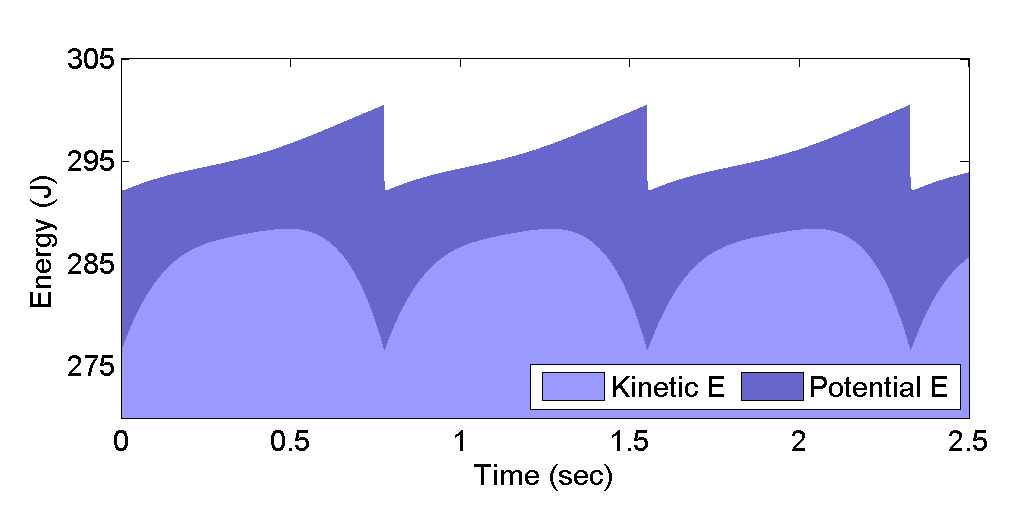
\includegraphics[width=1.0\columnwidth]{energy_cg2d_3link}
      \caption{Energy is not conserved as the controller injects energy.}
    \end{figure}
  }

  \only<3>{
    \begin{figure}
      \includemedia[
        width=1.0\columnwidth,
        height=0.5\columnwidth,
        addresource=cg2d_3link_simulation.mp4,
        activate=pageopen,
        flashvars={source=cg2d_3link_simulation.mp4&loop=true&autoPlay=true}
      ]{}{VPlayer9.swf}
      \caption{Stable passive gaits can be found for a range of slopes.}
    \end{figure}
  }

\end{frame}

\section{Orbital Stabilization}
\showtoc

\subsection{Orbital Stabilization with Control Lyapunov Functions}
\begin{frame}
  \frametitle{Orbital Stability}
  \begin{itemize}
  \item Periodic orbits have associated energy levels which define a hypersurface.
  \item We can stabilize to an energy level.
  \end{itemize}
\end{frame}


\begin{frame}
  \frametitle{Energy Shaping}
  Define the output $\eta = E_{c}(q, \dot q) - E_{0}$.
  Control Lyapunov Function
\end{frame}

\begin{frame}[t]
  \frametitle{Quadratic Programming}
  \begin{align}
    \nonumber
    \argmin_{v = (\delta, u)}  \, & v^T \! H \, v + h^T(q, \dot q) v\\
    \label{clf} \tag{clf}
    \mbox{s.t. } & A_{\mathit{clf}}(q, \dot q) v \leq b_{\mathit{clf}}(q, \dot q)\\
    \label{lim} \tag{lim}
    & A_{\mathit{lim}} v \leq b_{\mathit{lim}}
  \end{align}
  where
  \only<1>{
    \begin{itemize}
    \item\eqref{clf} imposes the control Lyapunv function
    \item\eqref{lim} imposes torque limits
    \end{itemize}
  }
  \only<2>{
    \begin{align*}
      H = \left(\begin{array}{c c}\epsilon & 0\\ 0 & I\end{array}\right), & \qquad
        h(q, \dot q) = \left(\begin{array}{c} 0\\ -2 \, \bar u(q, \dot q) \end{array}\right),\\
        A_{\mathit{clf}} = \left(\begin{array}{c c}
          -1 & 2 \eta L_{g} \eta
        \end{array}\right), & \qquad
        b_{\mathit{clf}} = -\epsilon \eta^{2} - 2\eta L_{f} \eta.
    \end{align*}
  }
  %The above acts to stabilize the energy of the system while attempting to obey the nominal system dynamics.
\end{frame}

\begin{frame}
  \frametitle{Example: Compass Gait as a Shaped System}
  \only<1>{
    \begin{columns}
      \column{1.5in}
      Dynamic Model:
      \begin{align*}
        M(q) \ddot q + H(q, \dot q) = 0
      \end{align*}
      Control Law:
      \begin{align*}
        \bar u(q) &= G(q) - G(\Psi(q)).
      \end{align*}

      \column{1.5in}
      \begin{figure}
        \centering
        \def\svgwidth{1.0\columnwidth}
        \input{figures/cg2d-2link-model.eps_latex}
        \vspace{-2em}
        \caption{Compass-gait biped with Controlled Symmetries.}
      \end{figure}
    \end{columns}
  }
  \only<2>{
    \begin{figure}
      \centering
      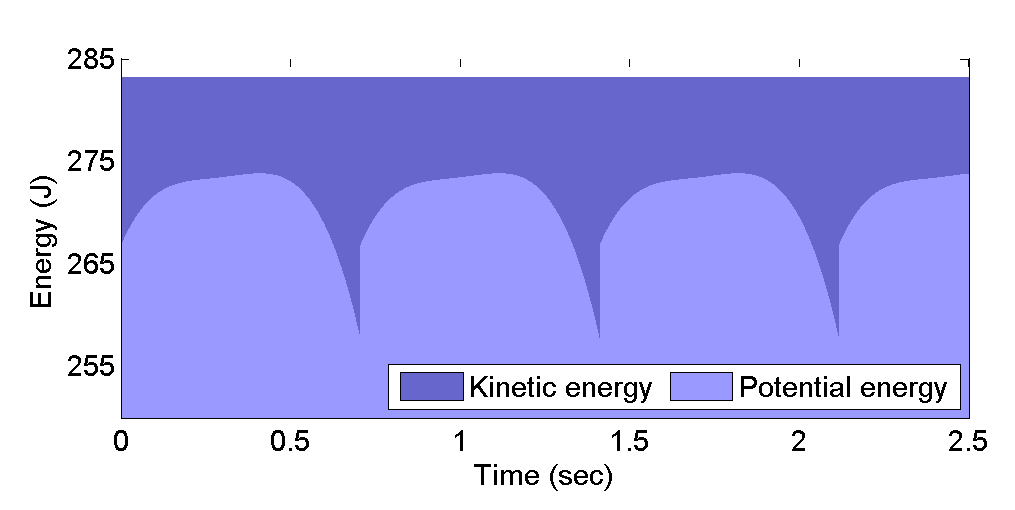
\includegraphics[width=1.0\columnwidth]{energy_cg2d_slope_model}
      \caption{Energy of the shaped system is conserved.}
    \end{figure}    
  }
  %  \only<3>{
  %    \includemedia[
  %      width=1.0\columnwidth,
  %      height=0.5625\columnwidth,
  %      addresource=amber2d.mp4,
  %      activate=pageopen,
  %      flashvars={source=amber2d.mp4&loop=true&autoPlay=true}
  %    ]{}{}%VPlayer9.swf}
  %  }

  \only<3>{
    Energy shaping can be achieved using:
    \begin{align}
      \nonumber
      \argmin_{v = (\delta, u)}  \, & v^T \! H \, v + h^T(q, \dot q) v\\
      \label{clf} \tag{clf}
      \mbox{s.t. } & A_{\mathit{clf}}(q, \dot q) v \leq b_{\mathit{clf}}(q, \dot q)
    \end{align}
    where
    \begin{align*}
      H = \left(\begin{array}{c c}\epsilon & 0\\ 0 & I\end{array}\right), \qquad
        h(q, \dot q) = \left(\begin{array}{c} 0\\ -2 \, \bar u(q, \dot q) \end{array}\right),
    \end{align*}
    and
    \begin{align*}
      A_{\mathit{clf}} = \left(\begin{array}{c c}
        -1 & 2 \eta L_{g} \eta
      \end{array}\right), \qquad
      b_{\mathit{clf}} = -\epsilon \eta^{2} - 2\eta L_{f} \eta
    \end{align*}
  }
\end{frame}


\begin{frame}
  \frametitle{Nonconservative Systems}
  nconsys
\end{frame}

\begin{frame}
  \frametitle{Example: 3-Link Biped}
  \only<2>{
    \begin{figure}
      \centering
      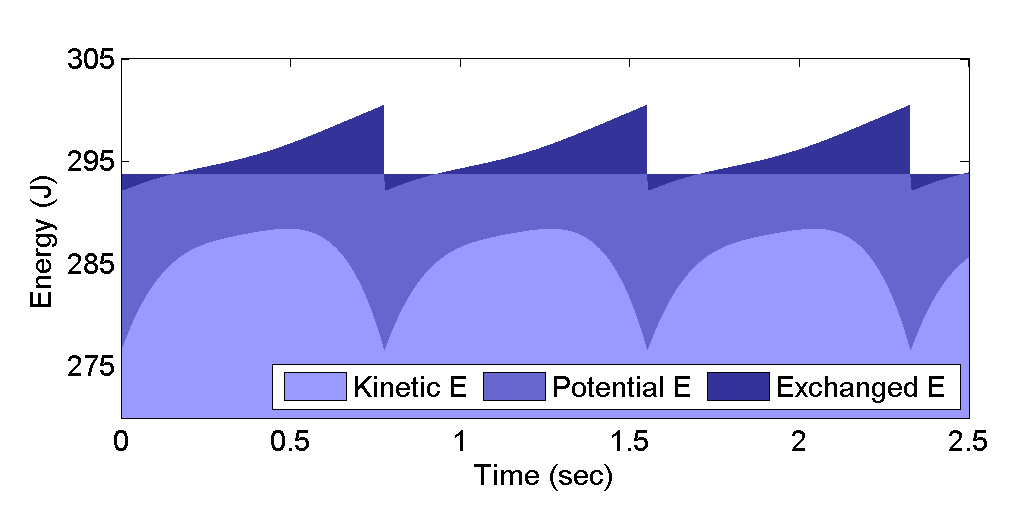
\includegraphics[width=1.0\columnwidth]{energy_conserved_cg2d_3link}
      \caption{The quantity, $E_{0} \equiv T(q, \dot q) + V(q) + \int_{0}^{t} F_{nc} \cdot dq$, is conserved.}
    \end{figure}
  }
\end{frame}

\section{Geometric Reduction}
\showtoc

\begin{frame}
  \frametitle{Overview}
  diagram
\end{frame}

\subsection{Functional Routhian Reduction}
\begin{frame}
  \frametitle{History}
  \begin{description}[D]
  \item[ Geometric reduction\footnote{For more on geometric reduction, see [Marsden, Springer-Verlag 1994]}:] \hspace{5cm}

    \begin{itemize}
    \item Begin with a Lagrangian $\Lagrangian : T\ConfigurationSpace \to \R$.
    \item Symmetries in the system are characterized by \textcolor{blue}{cyclic}
      variables: $\frac{\partial \Lagrangian}{\partial \phi} = 0$.
    \item The dimensionality of the phase space can be reduced (by ``dividing'' out by the symmetries).
    \item A corresponding Lagrangian, the \textcolor{blue}{Routhian}, can be defined on this reduced phase space.
    \end{itemize}
  \end{description}

  \begin{block}{Geometric Reduction ``Theorem''}
    One can understand the behavior of the full-order system in terms of
    the behavior of the reduced system and vice versa.
  \end{block}
\end{frame}

\begin{frame}
  \frametitle{Motivation}
  \begin{description}[D]
  \item[ Classical Reduction:]  The conserved quantities used to reduce and reconstruct systems are constants.
  \item[ Yet:]  It may be desirable to \alert{vary} the cyclic variables while not affecting the reduced order system.
  \item[ Motivates:]  An extension of Routhian reduction, termed \alert{functional Routhian reduction}, where the conserved quantities are functions of the cyclic variables:
    \begin{itemize}
    \item Allows us to control the cyclic variables.
    \item Can be effectively used to reduce bipedal robotic walkers.
    \item Generalizes to hybrid systems.
    \end{itemize}
  \end{description}
\end{frame}

\begin{frame}
  \frametitle{Almost-Cyclic Lagrangians \& Functional Routhians}
  \vspace{-1mm}

  Consider the case when $\ConfigurationSpace = S \times \S$ where $S$ is called the \textcolor{blue}{shape space}; we denote an element $q \in \ConfigurationSpace$ by $q = (\theta^T, \varphi)^T$.

  \vspace{-1mm}

  \begin{definition}
    A Lagrangian $\Llambda : TS \times T\S \to \R$ is \alert{almost-cyclic} if:
    \vspace{-3mm}
    \begin{align*}
      \Llambda(\theta, \phi, \dot \theta, \dot \phi)  =
      \frac{1}{2} \left(\!\!\begin{array}{cc}
      \dot \theta^T  &  \dot \phi
      \end{array}\!\!\right) \Mlambda(\theta)
      \left(\begin{array}{c}
        \dot \theta\\
        \dot \phi
      \end{array}\right) - \Wlambda(\theta, \phi, \dot \theta) - \Vlambda(\theta, \phi),
    \end{align*}
    for some function $\lambda : \S \to \R$.
  \end{definition}

  \only<1>{
    \vspace{-7mm}
    \textcolor{darkgray}{
      \begin{align*}
        \Mlambda(\theta) &= \left(\begin{array}{cc}
          \textcolor{lightblue}{\Mtheta(\theta)} + \Mphitheta^T(\theta) \Mphi^{-1}(\theta) \Mphitheta(\theta) & \Mphitheta^T(\theta)\\
          \Mphitheta(\theta) \qquad & \Mphi(\theta)
        \end{array}\right),\\[0mm]
        \Wlambda(\theta,\phi,\dot \theta) &= \textcolor{berkeleygold}{\lambda(\varphi)} \Mphi^{-1}(\theta) \Mphitheta(\theta) \dot{\theta},\\[0mm]
        \Vlambda(\theta,\phi) &= \textcolor{lightblue}{\Vt(\theta)} - \frac{1}{2} \textcolor{berkeleygold}{\lambda(\varphi)} \Mphi^{-1}(\theta) \textcolor{berkeleygold}{\lambda(\varphi)}.
      \end{align*}
    }
  }

  \only<2>{
    \begin{definition}
      The corresponding \alert{ functional Routhian} $\Lt : TS \to \R$ is: \vspace{-.3cm}
      \begin{eqnarray*}
        \Lt(\theta, \dot \theta) &=& \left[ \Llambda(\theta, \varphi, \dot{\theta}, \dot{\varphi}) - \lambda(\varphi) \dot{\varphi} \right]_{\Jfcn = \lambda(\varphi)}\\[0mm]
        & = &  \frac{1}{2} \dot{\theta}^T M_\theta(\theta) \dot{\theta} - \Vt(\theta).
      \end{eqnarray*}
    \end{definition}
  }
\end{frame}

\begin{frame}
  \frametitle{Functional Routhian Reduction}

  \begin{theorem}
    {\small Let $\Llambda$ be an almost-cyclic Lagrangian with an almost-cyclic variable, $\varphi$, and $\Lt$ the corresponding functional Routhian with shape space $S = \R^{n - 1}$. Let $\Upsilon : TS \times \S \to \R^n$ represent external forces satisfying:
      \begin{enumerate}
      \item $\Fextt$ does not depend on $\varphi,\dot{\varphi}$,
      \item $\Upsilon_i(\theta,\dot{\theta}) = 0$ for $i = 2, \ldots, n$.
      \end{enumerate}
      Then $(\theta(t), \varphi(t), \dot{\theta}(t), \dot{\varphi}(t))$ is a solution to the forced vector field $f_{\Llambda}$ on $[t_0, t_F]$ with \vspace{-2mm}
      \begin{align*}
        \dot{\varphi}(t_0) = \Mphi^{-1}(\theta(t_0)) (\lambda(\varphi(t_0)) - \Mphitheta(\theta(t_0))\dot{\theta}(t_0)),\\[-7mm]
      \end{align*}
      if and only if $(\theta(t), \dot{\theta}(t))$ is a solution to the forced vector field $f_{\Lt}$ and $(\varphi(t), \dot{\varphi}(t))$ satisfies:\vspace{-2mm}
      \begin{align*}
        \dot{\varphi}(t) = \Mphi^{-1}(\theta(t)) (\lambda(\varphi(t)) - \Mphitheta(\theta(t))\dot{\theta}(t)).\\[-1.2cm]
    \end{align*}}
  \end{theorem}
\end{frame}



%%%%
\subsection{Reduction Control Laws}
\frame[t] {
  \frametitle{Sagittal Control Law: Reduced Dynamics Controller}

  Consider the sagittal restriction of the 3D biped, which will be a 2D biped, and apply a 2D controller that results in stable walking for this system.

  \only<1> {
    \begin{columns}
      \begin{column}{0.3\textwidth}
        \begin{figure}
          \centering
          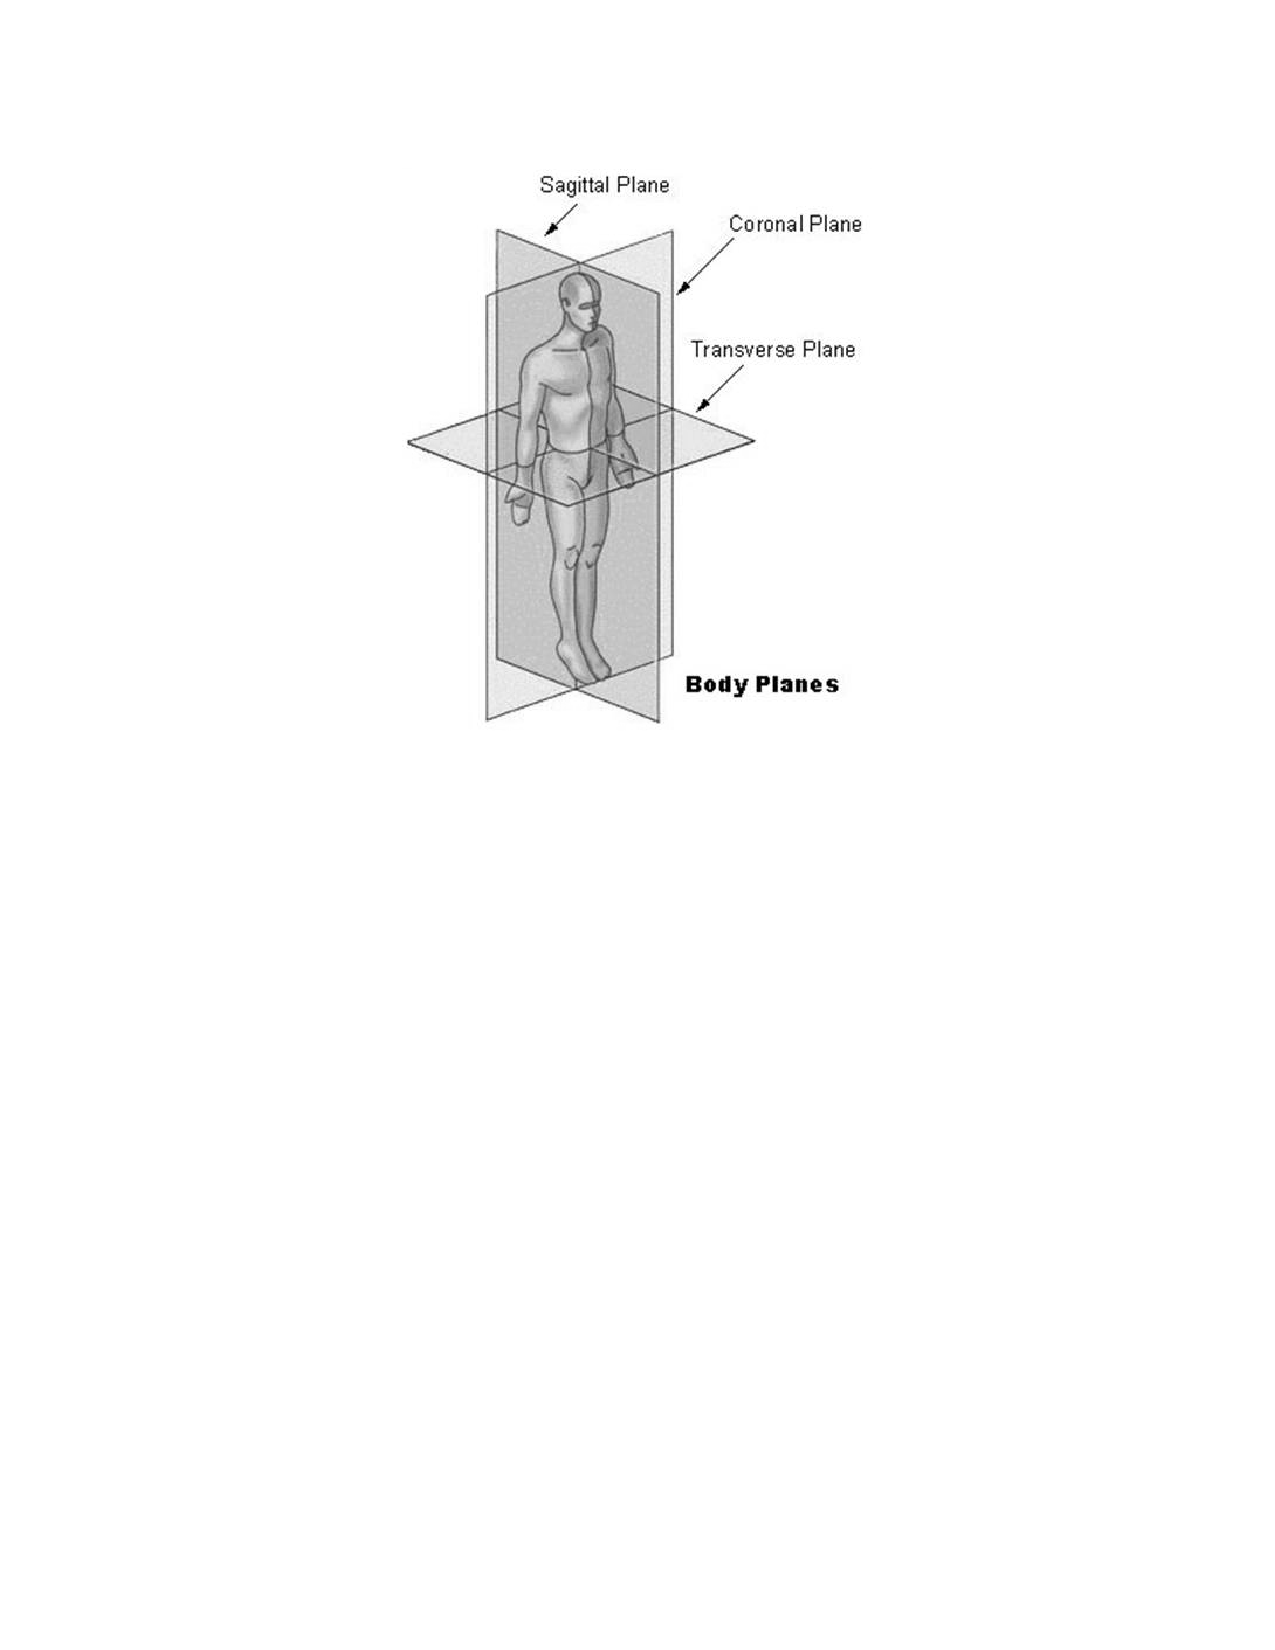
\includegraphics[height=4cm]{bodyplanes}
        \end{figure}
      \end{column}
      \begin{column}{0.6\textwidth}
        \begin{figure}
          \centering
          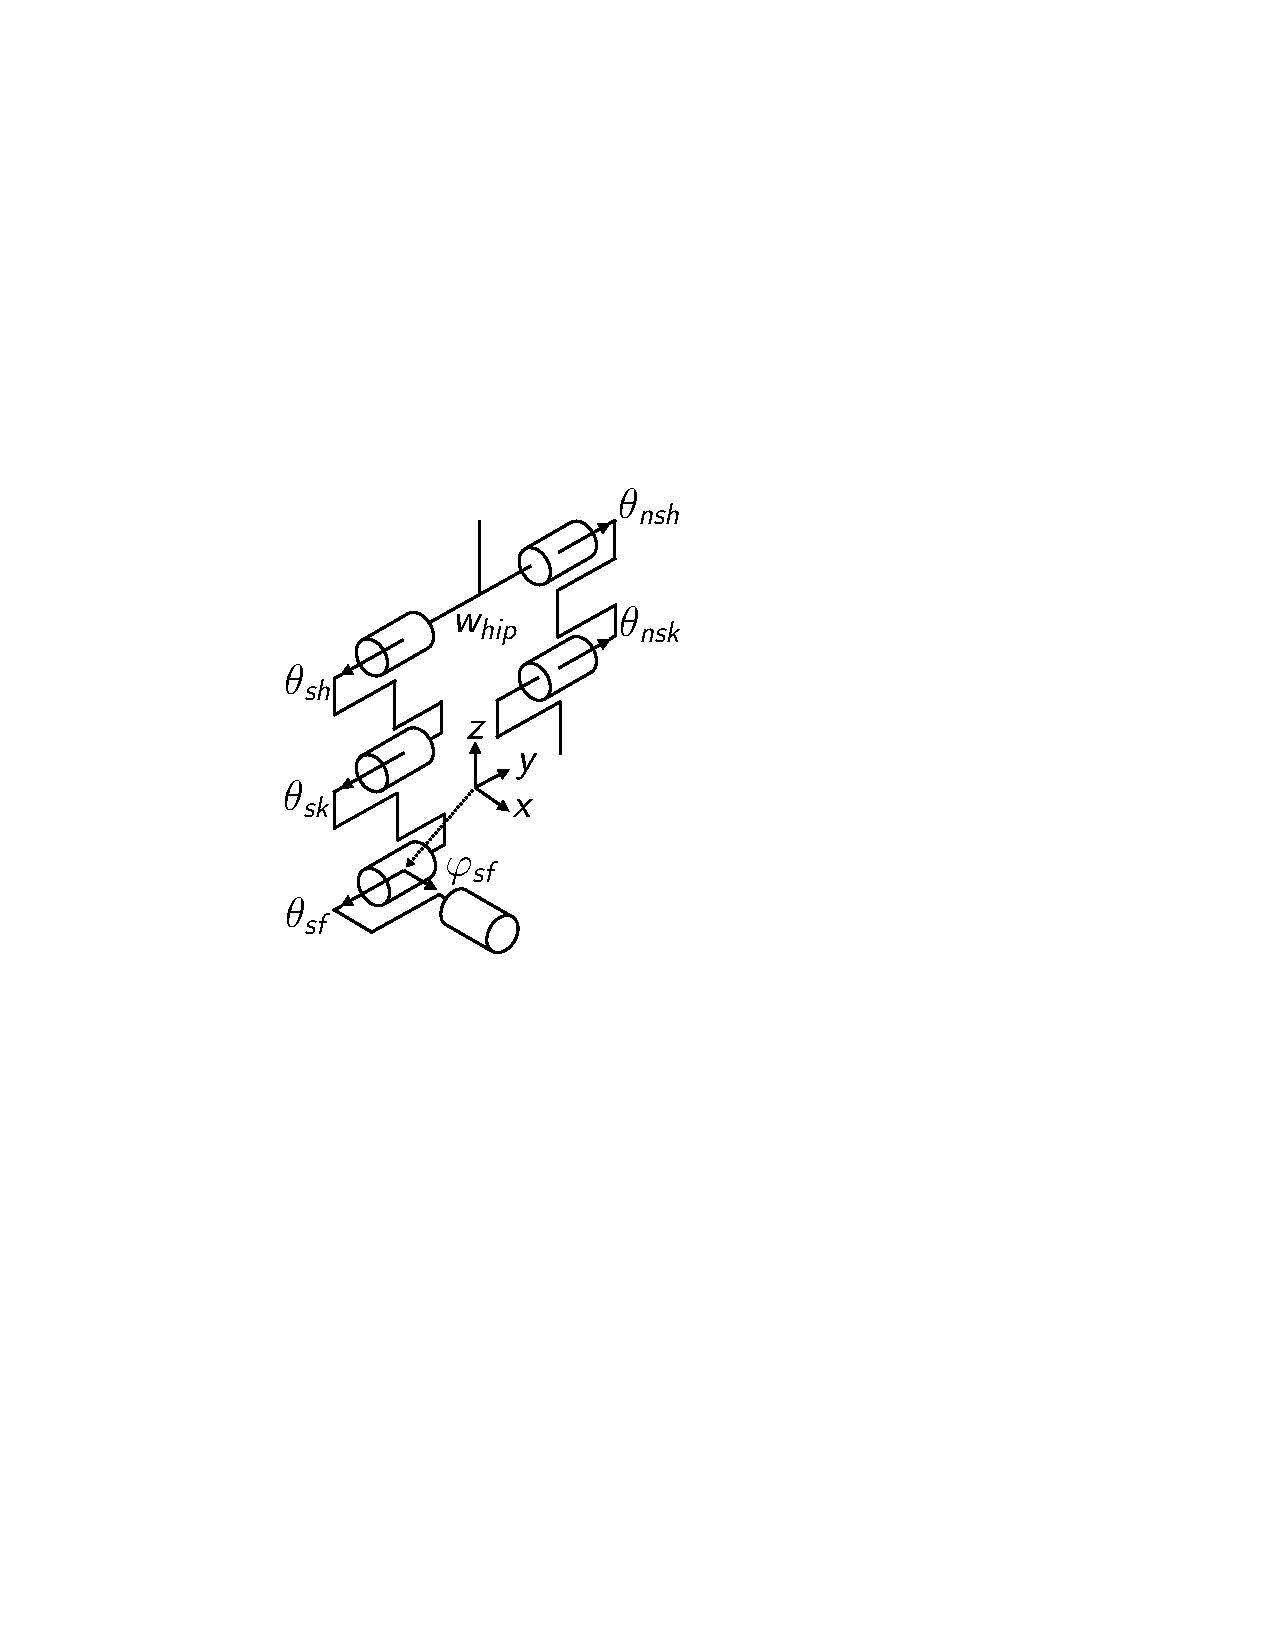
\includegraphics[height=3cm]{robot_angles_3d} \qquad
          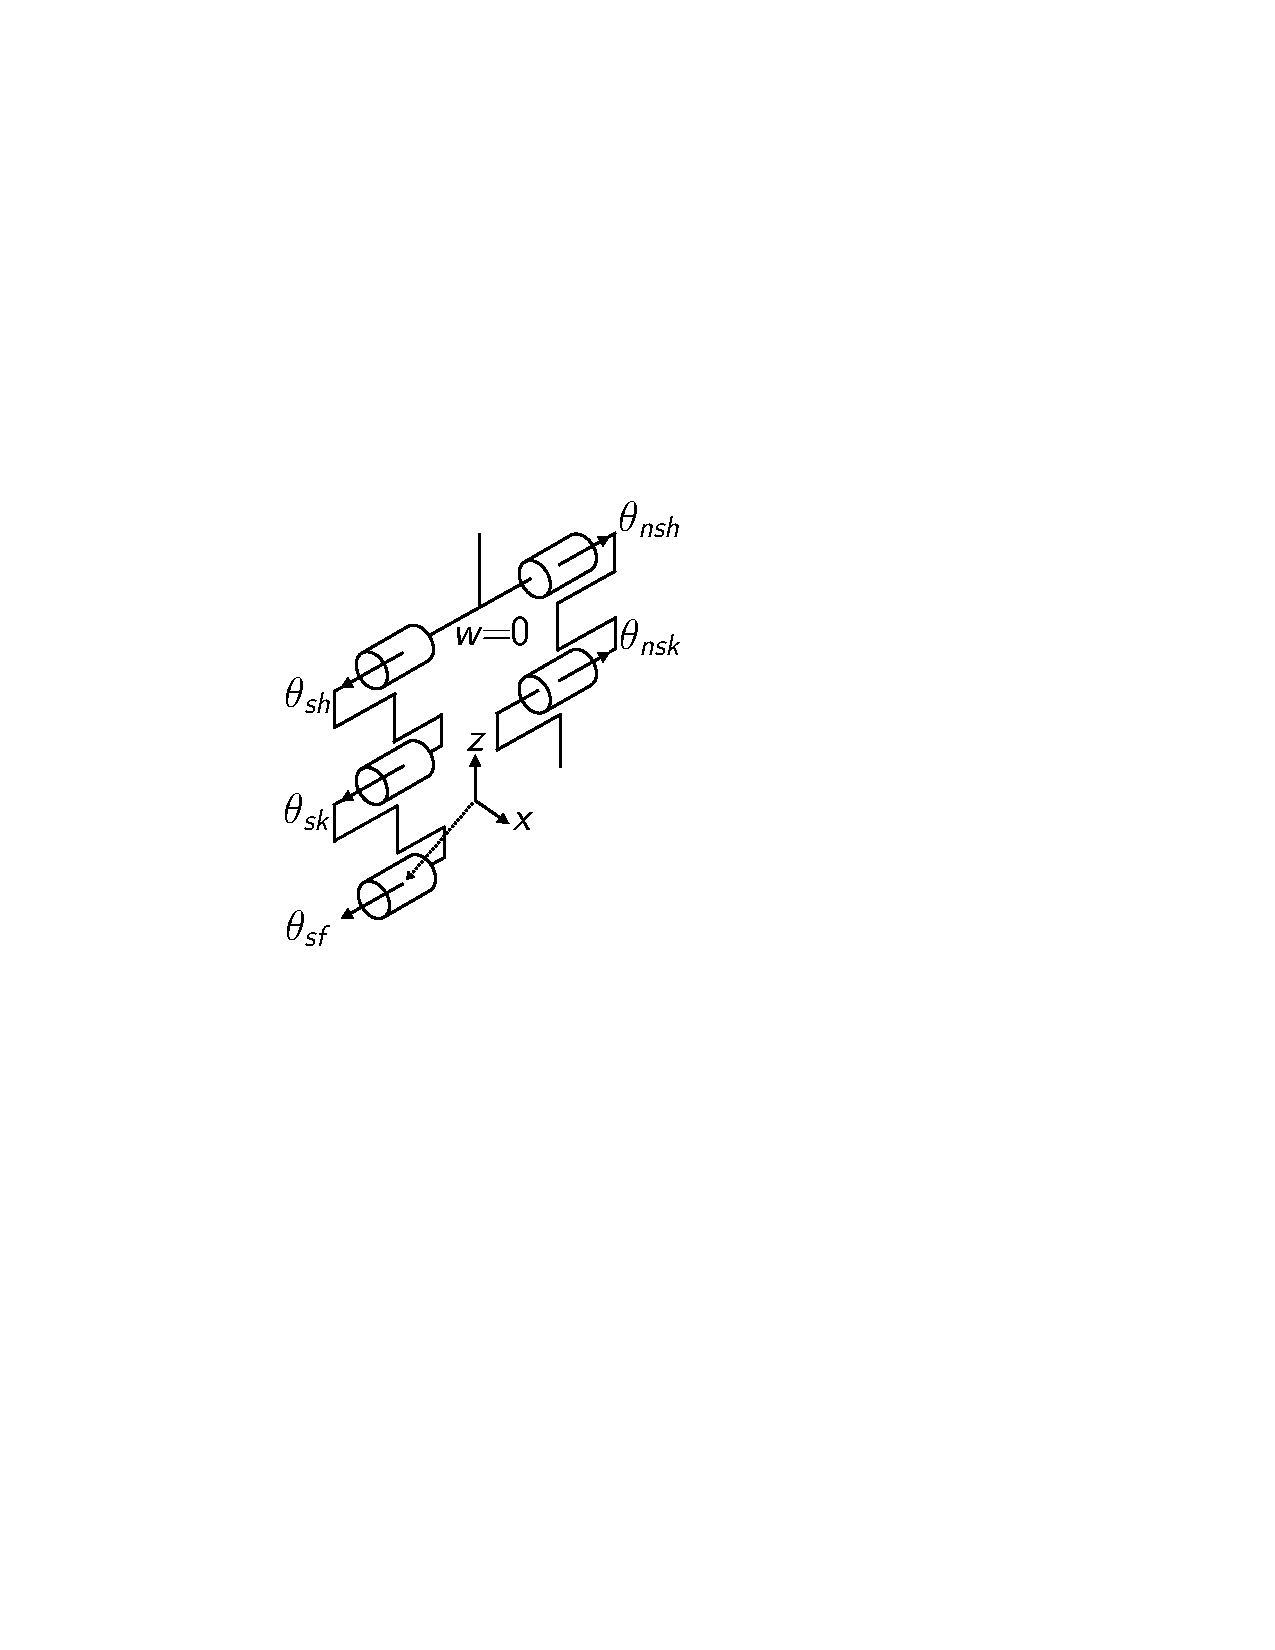
\includegraphics[height=3cm]{robot_angles_2d}
          \caption{Sagittal restriction of of 3D biped leads to a reduced model.}
        \end{figure}
      \end{column}
    \end{columns}
  }

  \only<2> {
    {\scriptsize  \textcolor{gray}{
        \begin{diagram}[width=5em,height=5em]
          \textcolor{black}{\fbox{$\begin{array}{c}$Hipped 3D Biped$\end{array}$}} &
          \rTo^{1^{\mathsf{st}} \:\: \mathsf{Reduction}}_{\mathsf{Control} \:\: \mathsf{Law}} &
          \fbox{$\begin{array}{c}$3D Biped$\\$with shaped$\\$energy$\end{array}$} &
          \rTo^{2^{\mathsf{nd}} \:\: \mathsf{Reduction}}_{\mathsf{Control} \:\: \mathsf{Law}} &
          \fbox{$\begin{array}{c}$3D Biped$\\$walking stably$\end{array}$}\\
          \dDashto^{\textcolor{black}{\mathsf{Sagittal}}}_{\textcolor{black}{\mathsf{Restriction}}} &&
          \uTo \dTo_{\begin{array}{c}$Reduction$\end{array}}&&\\
          \textcolor{black}{\fbox{$\begin{array}{c}$2D Biped$\end{array}$}} &
          \rTo^{\textcolor{black}{\mathsf{Sagittal}}}_{\textcolor{black}{\mathsf{Control} \:\: \mathsf{Law}}} &
          \textcolor{black}{\fbox{$\begin{array}{c}$2D Biped$\\$walking stably$\end{array}$}} && \\
    \end{diagram}}}
  }

  \only<3> {
    \begin{itemize}
    \item  The Lagrangian of the 3D biped has the general form:
      \begin{eqnarray}
        \label{eq:submats}
        \lefteqn{\Lfd(\cq{},\cdq{}) = -\Vu \ + }\\
        \nonumber
        &&\frac{1}{2}
        \left(\begin{array}{c c}
          \dot{\theta}^T & \dot{\varphi}
        \end{array}\right)
        \underbrace{\left(\begin{array}{c c}
            \Mth & \Mphitheta^T(\theta,\varphi)\\
            \Mphitheta(\theta,\varphi) & \Mphi(\theta,\varphi)
          \end{array}\right)}_{\mMu}
        \left(\begin{array}{c}
          \dot{\theta}\\
          \dot{\varphi}
        \end{array}\right), \nonumber
      \end{eqnarray}
      \vspace{-5mm}

    \item The Lagrangian of the sagittal restriction is given by:
      \begin{align*}
        \Lrd(\theta,\dot{\theta}) = \frac{1}{2} \dot{\theta}^T \Mth \dot{\theta} - \left.\Vu\right\vert_{\varphi=0},
      \end{align*}

    \end{itemize}
  }

  \only<4> {
    \vspace{-.1cm}
    \begin{itemize}

    \item The Lagrangian of the sagittal restriction is given by:
      \begin{align*}
        \Lrd(\theta,\dot{\theta}) = \frac{1}{2} \dot{\theta}^T \Mth \dot{\theta} - \left.\Vu\right\vert_{\varphi=0},
      \end{align*}

    \item This yields a control system: $(\fr,\gr)$.

    \item \alert{Assume} there exists a control law, $\usagarg$, that results in stable 2D waking for the dynamical system:
      \begin{align*}
      \flt = \fr(\theta, \dot{\theta}) + \gr(\theta) \usagarg.
      \end{align*}

    \end{itemize}
  }

%\only<5> {
%  \begin{figure}
%    \centering
%    \movie[width=0.6\textwidth,externalviewer]{
%    \includegraphics[width=0.6\textwidth]{2dwalkinggait.pdf}}{Movies/2d-movie.avi}\\
%    \includegraphics[height=0.3\textheight]{pp-2d-legs.pdf}
%    \includegraphics[height=0.3\textheight]{pp-2d-feet.pdf}
%  \end{figure}
%}
%
}

\frame[t] {
  \frametitle{$1^{\mathsf{st}}$ Reduction Control Law: Lagrangian Shaping Controller}

  Shape the total energy of the 3D biped so that functional Routhian reduction can be applied and the reduced system is exactly the 2D system obtained from the first control law.

  {\scriptsize \textcolor{gray}{
      \begin{diagram}[width=5em,height=5em]
        \textcolor{black}{\fbox{$\begin{array}{c}$Hipped 3D Biped$ \end{array}$}} &
        \rTo^{\textcolor{black}{1^{\mathsf{st}} \:\: \mathsf{Reduction}}}_{\textcolor{black}{\mathsf{Control} \:\: \mathsf{Law}}} &
        \textcolor{black}{\fbox{$\begin{array}{c}$3D Biped$\\$with shaped$\\$energy$\end{array}$}} &
        \rTo^{2^{\mathsf{nd}} \:\: \mathsf{Reduction}}_{\mathsf{Control} \:\: \mathsf{Law}} &
        \fbox{$\begin{array}{c}$3D Biped$\\$walking stably$\end{array}$}\\
        \dDashto^{\textcolor{black}{\mathsf{Sagittal}}}_{\textcolor{black}{\mathsf{Restriction}}} &&
        \uTo \dTo_{\textcolor{black}{\begin{array}{c}$Reduction$\end{array}}}&&\\
        \textcolor{black}{\fbox{$\begin{array}{c}$2D Biped$\end{array}$}} &
        \rTo^{\textcolor{black}{\mathsf{Sagittal}}}_{\textcolor{black}{\mathsf{Control} \:\: \mathsf{Law}}} &
        \textcolor{black}{\fbox{$\begin{array}{c}$2D Biped$\\$walking stably$\end{array}$}} &&
      \end{diagram}
  }}
}


\frame[t] {
  \frametitle{$2^{\mathsf{nd}}$ Reduction Control Law: Zero Dynamics Controller}

  Use feedback linearization to stabilize to the surface of initial conditions for which the decoupling promised by functional Routhian Reduction is valid.

  {\scriptsize  \textcolor{gray}{
      \begin{diagram}[width=5em,height=5em]
        \textcolor{black}{\fbox{$\begin{array}{c}$Hipped 3D Biped$\end{array}$}} &
        \rTo^{\textcolor{black}{1^{\mathsf{st}} \:\: \mathsf{Reduction}}}_{\textcolor{black}{\mathsf{Control} \:\: \mathsf{Law}}} &
        \textcolor{black}{\fbox{$\begin{array}{c}$3D Biped$\\$with shaped$\\$energy$\end{array}$}} &
        \rTo^{\textcolor{black}{2^{\mathsf{nd}} \:\: \mathsf{Reduction}}}_{\textcolor{black}{\mathsf{Control} \:\: \mathsf{Law}}} &
        \textcolor{black}{\fbox{$\begin{array}{c}$3D Biped$\\$walking stably$\end{array}$}}\\
        \dDashto^{\textcolor{black}{\mathsf{Sagittal}}}_{\textcolor{black}{\mathsf{Restriction}}} &&
        \uTo \dTo_{\textcolor{black}{\begin{array}{c}$Reduction$\end{array}}}&& \\
        \textcolor{black}{\fbox{$\begin{array}{c}$2D Biped$\end{array}$}} &
        \rTo^{\textcolor{black}{\mathsf{Sagittal}}}_{\textcolor{black}{\mathsf{Control} \:\: \mathsf{Law}}} &
        \textcolor{black}{\fbox{$\begin{array}{c}$2D Biped$\\$walking stably$\end{array}$}}&&
      \end{diagram}
  }}
}

%%%%%%%%%%%%%%%%%%%%%%%%%%%%%%

\section{Human-Inspired Control}
\showtoc

\subsection{Human-Inspired Control Framework}
\frame{
  \frametitle{Human Data Experiment}
  \begin{columns}
    \begin{column}{0.65\textwidth}
      \begin{figure}
        \centering
        \vspace{-1cm}
        \caption{Experimental setup showing sensor placement for human data acquisition}
        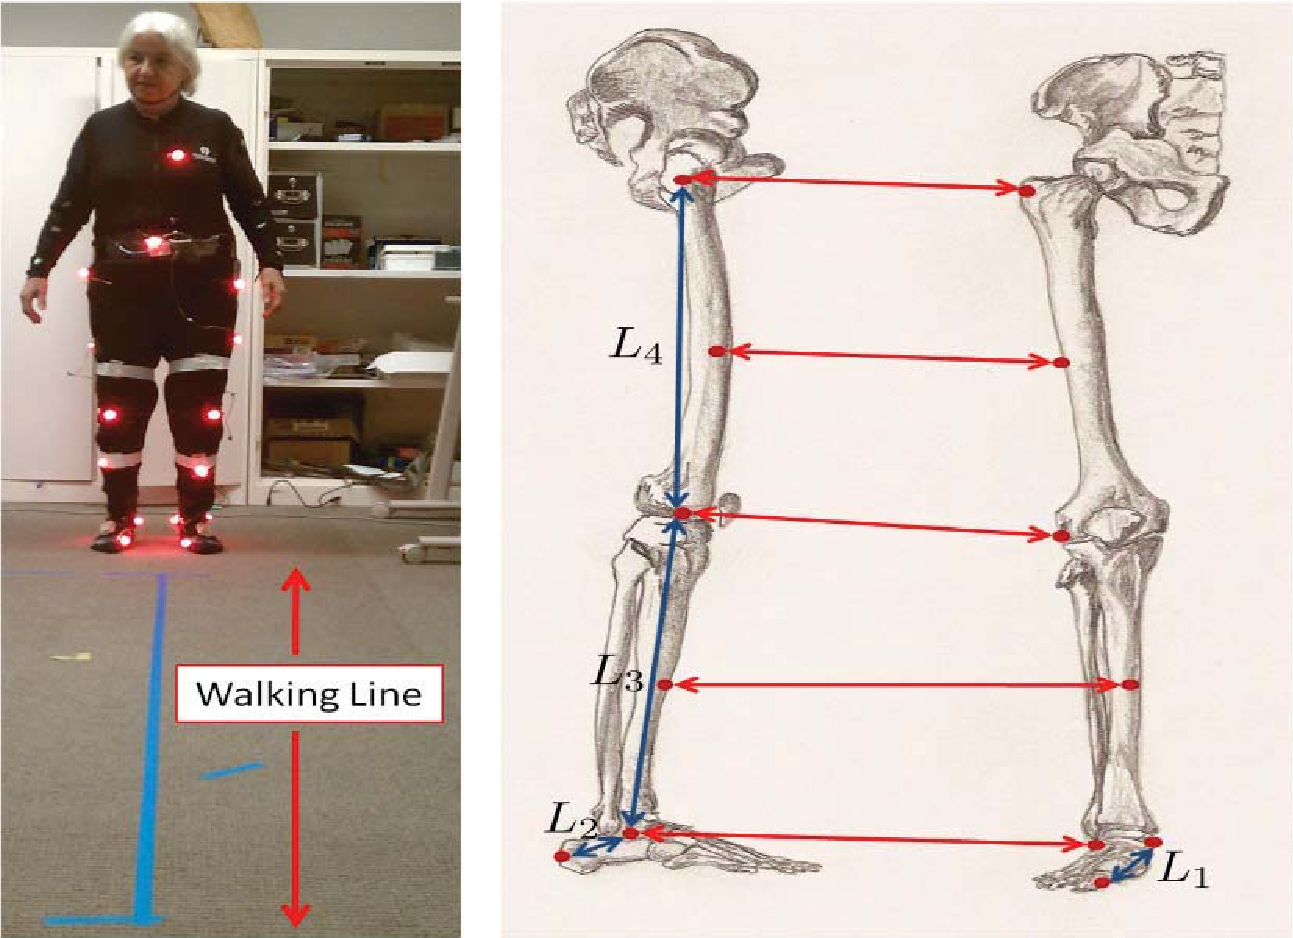
\includegraphics[width=1.0\columnwidth]{labeled_diagram}
      \end{figure}
    \end{column}
    \begin{column}{0.35\textwidth}
      \begin{figure} \centering
        \vspace{-1cm}
        \caption{Human outputs}
        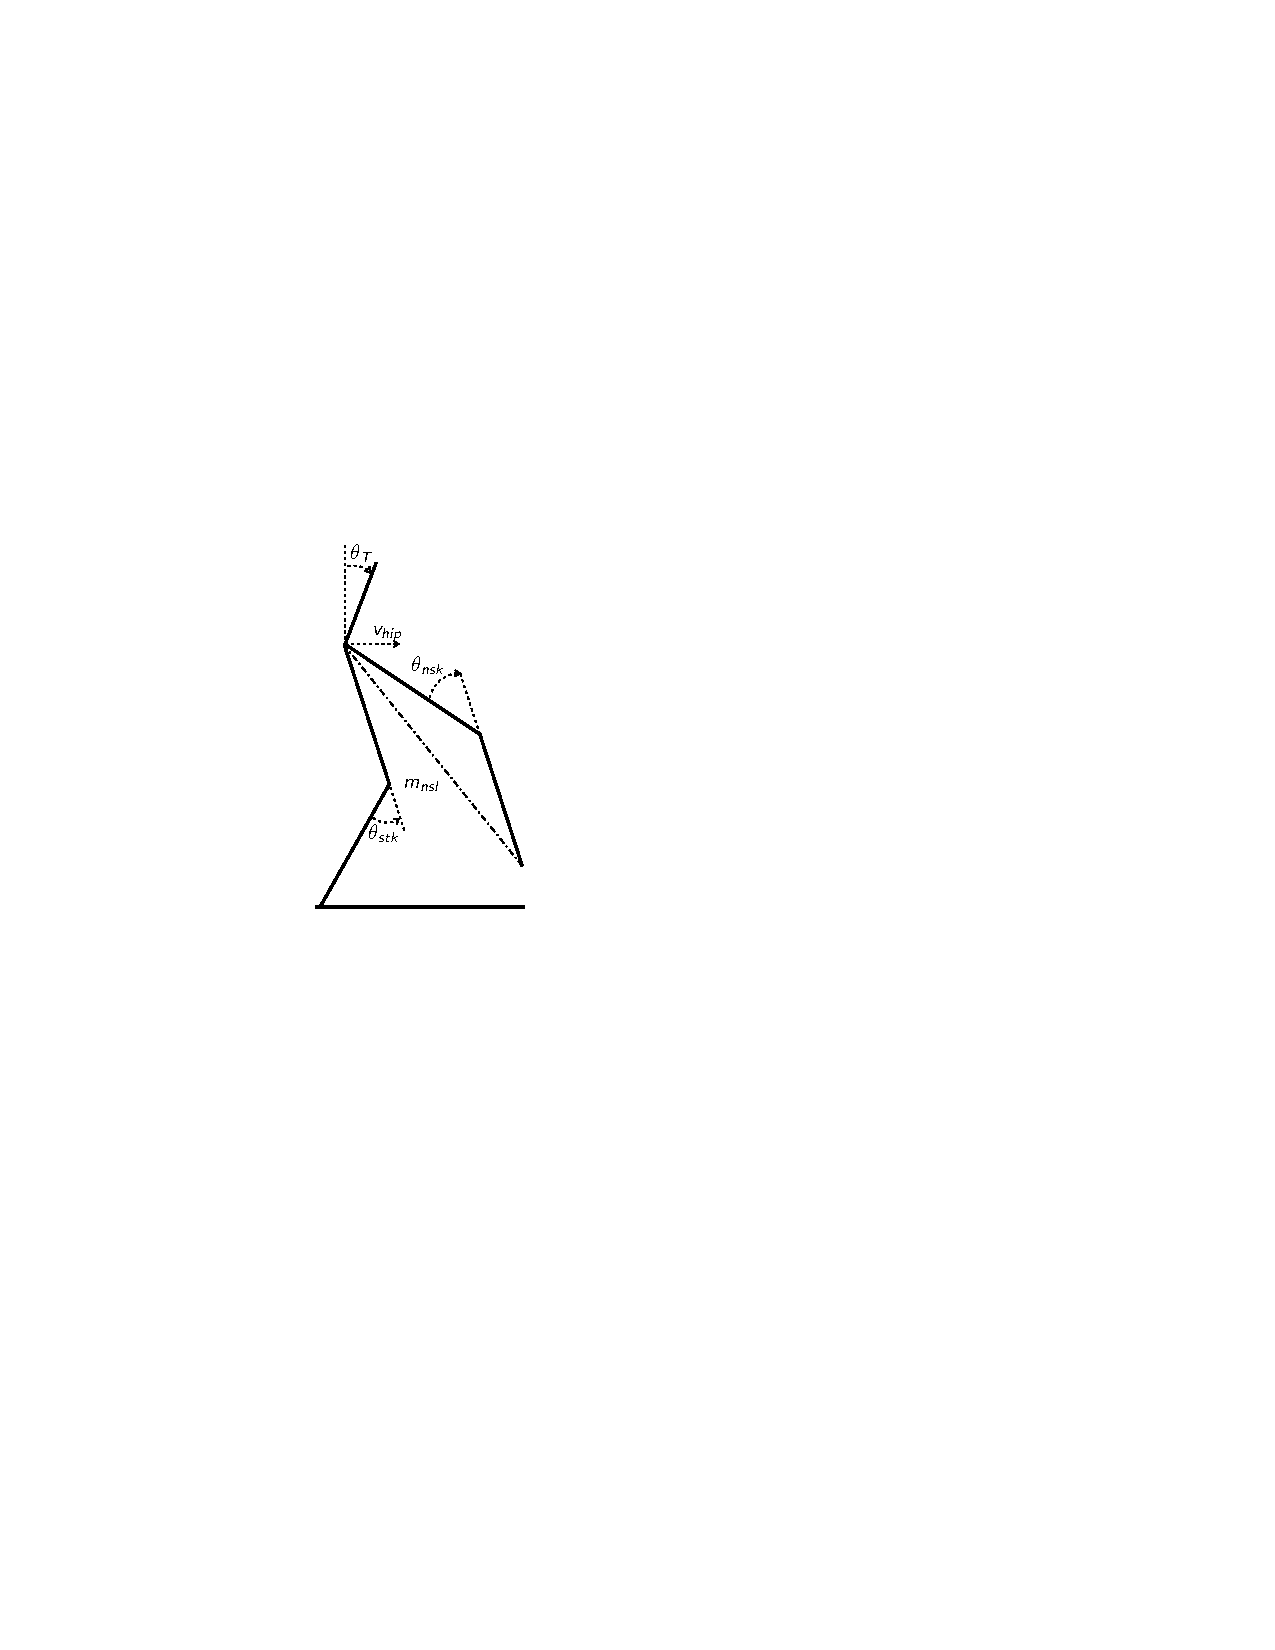
\includegraphics[width=0.8\columnwidth]{robot_const}
      \end{figure}
    \end{column}
  \end{columns}
}

\frame[t]{
  \frametitle{Canonical Walking Functions}
  The following function, termed a {\em canonical walking function}, fits human kinematics data quite accurately:
  \begin{align}
    \nonumber
    y(t) &= e^{-\zeta \omega_{n} t} (c_{1} \cos (\omega_{d} t) + c_{2} \sin (\omega_{d} t)) + \hat{g}\\
    \tag{CWF}
    \label{eq:cwf}
    y^{H}(t, A)&= e^{-a_{3} t} (a_{1} \cos (a_{2} t) + a_{4} \sin (a_{2} t)) + a_{5}
  \end{align}
  where,
  \begin{itemize}
  \item
    $\zeta$ is the damping ratio,
  \item
    $\omega_{n}$, $\omega_{d}$ are the natural and damped natural frequencies, resp.,
  \item
    $c_{1}$ and $c_{2}$ are initial conditions,
  \item
    and $\alpha$ and $\hat{g}$ are from a particular solution for certain forcing.
  \end{itemize}
  Parameterize time using hip position:
  \begin{align*}
    \tau(\theta) := \frac{p_\mathit{hip}^{x}(\theta) - p_\mathit{hip}^{x}(\theta^{-})}{v_\mathit{hip}}
  \end{align*}
}

\frame{
  \frametitle{Selecting Human Outputs}
  The following human kinematics outputs were selected:
  \begin{enumerate}
    {
    \item[\HF{1}:] $\Oa$, {\em forward hip velocity}, i.e., the velocity of the $x$-position of the hip,
    \item[\HF{2}:] $\Ob$, {\em swing leg slope}, i.e., the tangent of the angle between the $z$-axis and the projection of the line connecting the swing ankle and hip,
    \item[\HF{3}:] $\Oc$, {\em stance knee relative angle},
    \item[\HF{4}:] $\Od$, {\em swing knee relative angle},
    \item[\HF{5}:] $\Oe$, {\em vertical torso angle}, the angle of the torso measured with respect to the vertical axis of the world frame.
    }
  \end{enumerate}

  \vspace{1mm}
  For convenience, define the actual and desired outputs:
  \vspace{-1mm}
  \begin{align*}
    y_{1}^{a} = \Oa, \ y_{2}^{a} = \Ob, \ y_{3}^{a} = \Oc, \ y_{4}^{a} = \Od, \ y_{5}^{a} = \Oe,
  \end{align*}
  \vspace{-8mm}
  \begin{align*}
    y_{1}^{d} = y^{H}(\tau(\theta), A_1), \ \ldots, \ y_{5}^{d} = y^{H}(\tau(\theta), A_5)
  \end{align*}
}

\frame{
  \frametitle{Human-Inspired Optimization}
  The form of \eqref{eq:cwf} allows it to encode certain outputs:
\vspace{-4mm}
  \begin{figure}
    \centering
    \caption{Canonical walking functions with parameters from \eqref{eq:opt}}
    \vspace{-2mm}
    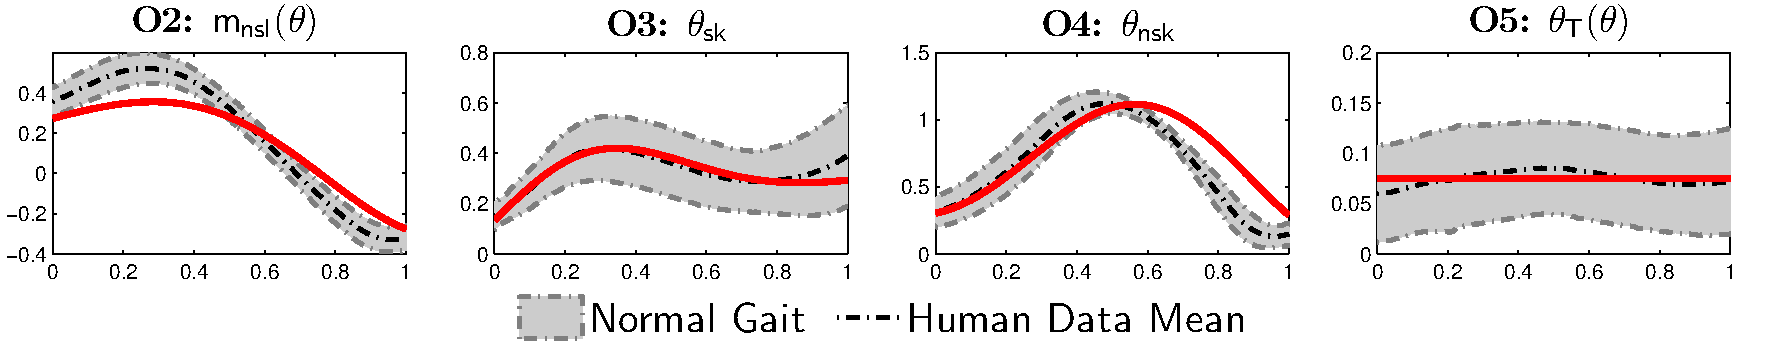
\includegraphics[width=1.0\textwidth]{human_function_fits}
    \vspace{-2mm}
  \end{figure}
  These outputs can be used to construct a {\em partial hybrid zero dynamics} parameterized by matrix A where outputs \textcolor{blue}{\HF{2}}--\textcolor{blue}{\HF{5}} of the robot and their derivatives are equal to the desired outputs for all time. The optimal parameters $A^*$ are found by solving
  \begin{align}
    \label{eq:opt}
    \tag{$\mathcal{O}$}
    A^{*} = \underset{A \in \R^{5 \times 5}}{\operatorname{argmin}} &  \:\: \mathrm{Cost}_{\mathrm{HD}}(A)  \\[-1mm]
    \nonumber
    \mathrm{s.t.} \quad & \ResetMapReduced(\GuardReduced \cap \HZD_{A}) \subset \PHZD_{A}
  \end{align}
}

\frame {
  \frametitle{Tracking the Partial Hybrid Zero Dynamics}
  Instead of feedback linearization, use PD control as this will allow the reduction scheme posed in this paper to work properly:
  \begin{align*}
    \mathcal{K}_{2D}(\theta, \dot{\theta}) \! = \! k_p \left(\!\!
    \begin{array}{c}
      0\\
      y_{d,2} - y_{a,2}\\
      y_{d,3} - y_{a,3}\\
      y_{d,4} - y_{a,4}\\
      y_{d,5} - y_{a,5}
    \end{array}\!\!\right)  + 
    \blkdiag (k_p, k_d I_4)\left(\!\!
    \begin{array}{c}
      y_{d,1} - y_{a,1}\\
      \dot{y}_{d,2} - \dot{y}_{a,2}\\
      \dot{y}_{d,3} - \dot{y}_{a,3}\\
      \dot{y}_{d,4} - \dot{y}_{a,4}\\
      \dot{y}_{d,5} - \dot{y}_{a,5}
    \end{array}\!\!\right)
  \end{align*}

  This control law will result in walking in simulation (and in experiment in other works) and will satisfy assumptions made by functional Routhian reduction (introduced later).
}

%%%%%%%%%%%%%%%%%%%%%%%

\section{Conclusions}
\showtoc

\subsection{Remaining Work and Concluding Remarks}
\begin{frame}
  \frametitle{Current Results}
  \begin{itemize}
  \item 2D Compass-gait
  \item 2D 3-link
  \item 3D 3-link
  \item 2D 7-link
  \item 2D 5-link with HIC
  \end{itemize}
\end{frame}

\begin{frame}
  \frametitle{Remaining Work}
  \begin{itemize}
  \item 3D 5-link ES+HIC+FRR
  \item Formal proof of energy shaping
  \item 3D 7-link
  \end{itemize}
\end{frame}

\begin{frame}
  \frametitle{Walking with Feet}
  \begin{itemize}
  \item 2D biped with feet
  \end{itemize}
\end{frame}

%% \section{Conclusions}
%% \showtoc
%% \begin{frame}
%%   \frametitle{Conclusions}
%%   con.
%% \end{frame}

%\section{Hybrid Systems}
%
%\subsection{Formalisms}
%\frame{hsys}
%
%\section{Hybrid Models}
%\frame{hmodels}
%
%\section{Controlled Lagrangians}
%\begin{frame}
%  \begin{itemize}
%    \item Explain the significance of energy in mechanical systems.
%  \end{itemize}
%\end{frame}

%\section{Energy Shaping}
%\frame{ES}
%\begin{frame}
%  \frametitle{Formulation}
%  s
%\end{frame}


%% \begin{frame}
%%   \frametitle{A Simple Example}
%%   The pendulum can be stabilized to a given level set of the energy.
%% \end{frame}
%% 


\end{document}
